\begin{minted}[]{r}
library(ggplot2)
ggplot(diamonds, aes(x = carat, fill = color)) +
        geom_histogram(bins = 30)
\end{minted}

\begin{figure}[H]

{\centering 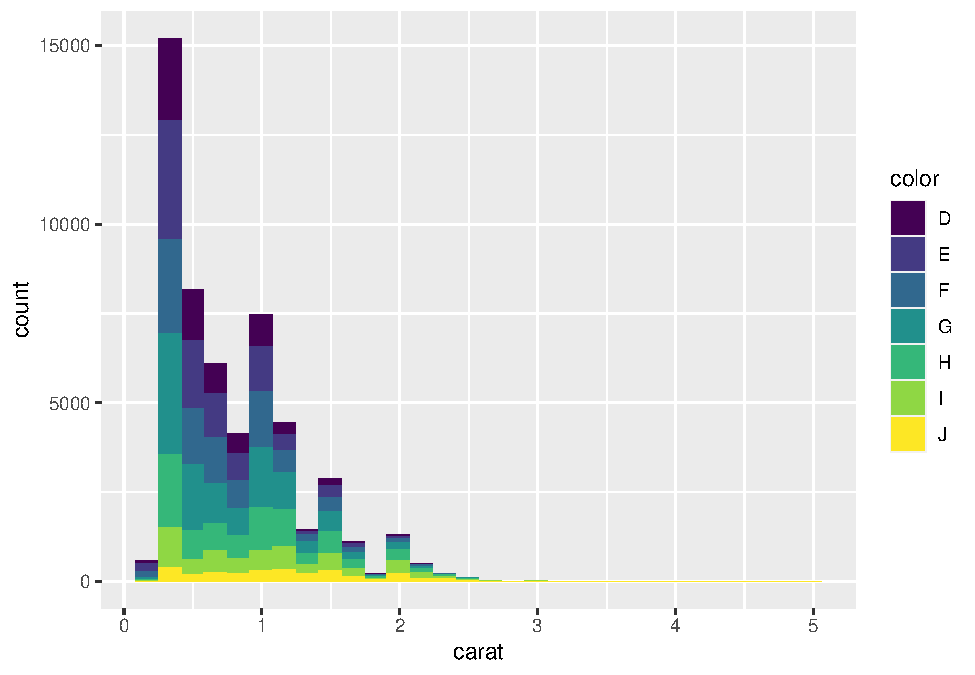
\includegraphics[width=0.75\linewidth]{../images/figs/chunk1-1} 

}

\caption{\label{fig:fig1}Plot 1}\label{fig:chunk1}
\end{figure}

Figure \ref{fig:fig1} shows that\ldots{}

\pagebreak

\begin{minted}[]{r}
ggplot(diamonds, aes(x = carat, y = price)) +
    geom_point(aes(color = cut)) +
    geom_smooth()
\end{minted}

\begin{figure}[H]

{\centering 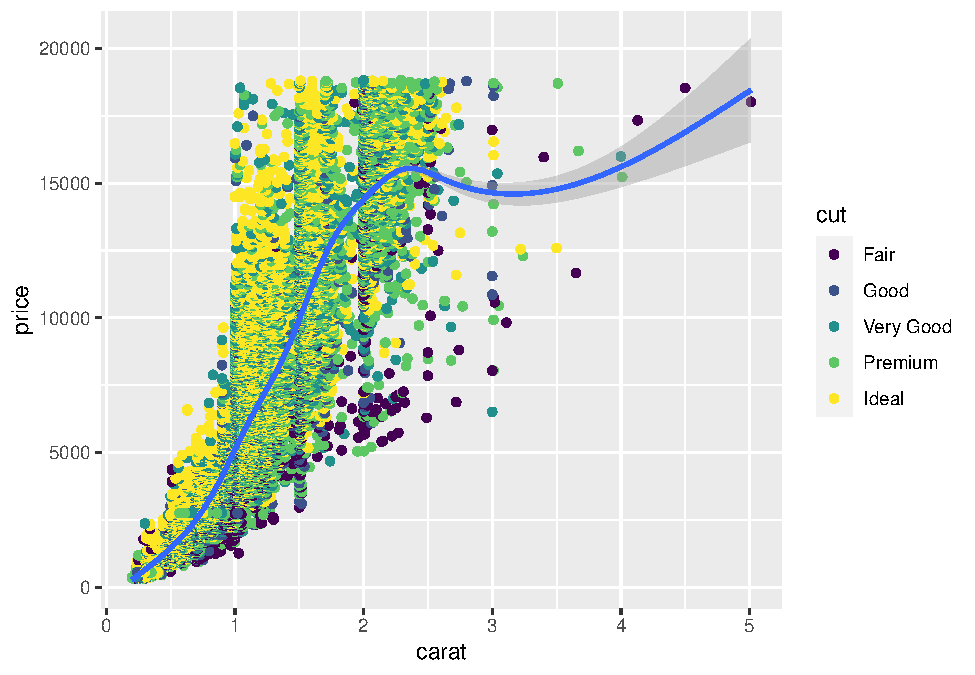
\includegraphics[width=0.75\linewidth]{../images/figs/chunk2-1} 

}

\caption{\label{fig:fig2}Plot 1}\label{fig:chunk2}
\end{figure}

Figure \ref{fig:fig2} instead shows that\ldots{}
